\section{Abstandsregler}
\subsection{Simulink-Modell}
Für den Abstandsregelung werden die zuvor beschrieben Objekterkennung und die Matrixtransformation genutzt. 
Aus dem RGB-Eingangsvideosignal wird der Rotkanal durch Subtraktion der beiden anderen Kanäle extrahiert und anschlie{\ss}- end in ein Schwarzwei{\ss}bild konvertiert.
 
In der \textit{finderechteck}-Funktion werden die vier Eckpunkte des Quadrats ermittelt. Dabei wird nur ein Signal weiterleitet, wenn ein Quadrat gefunden wurde. 

Mit der vorher definierten Höhe des Quadrats über dem Boden,   den Kameraparametern und der Transformationsmatrix können die Weltkoordinaten der beiden unteren getrackten Punkte bestimmt werden. Nach der Mittlung und Trennung der Signale wird die \textit{x}-, und \textit{y}-Position ausgegeben. 



\begin{figure}[h]
	\centering
	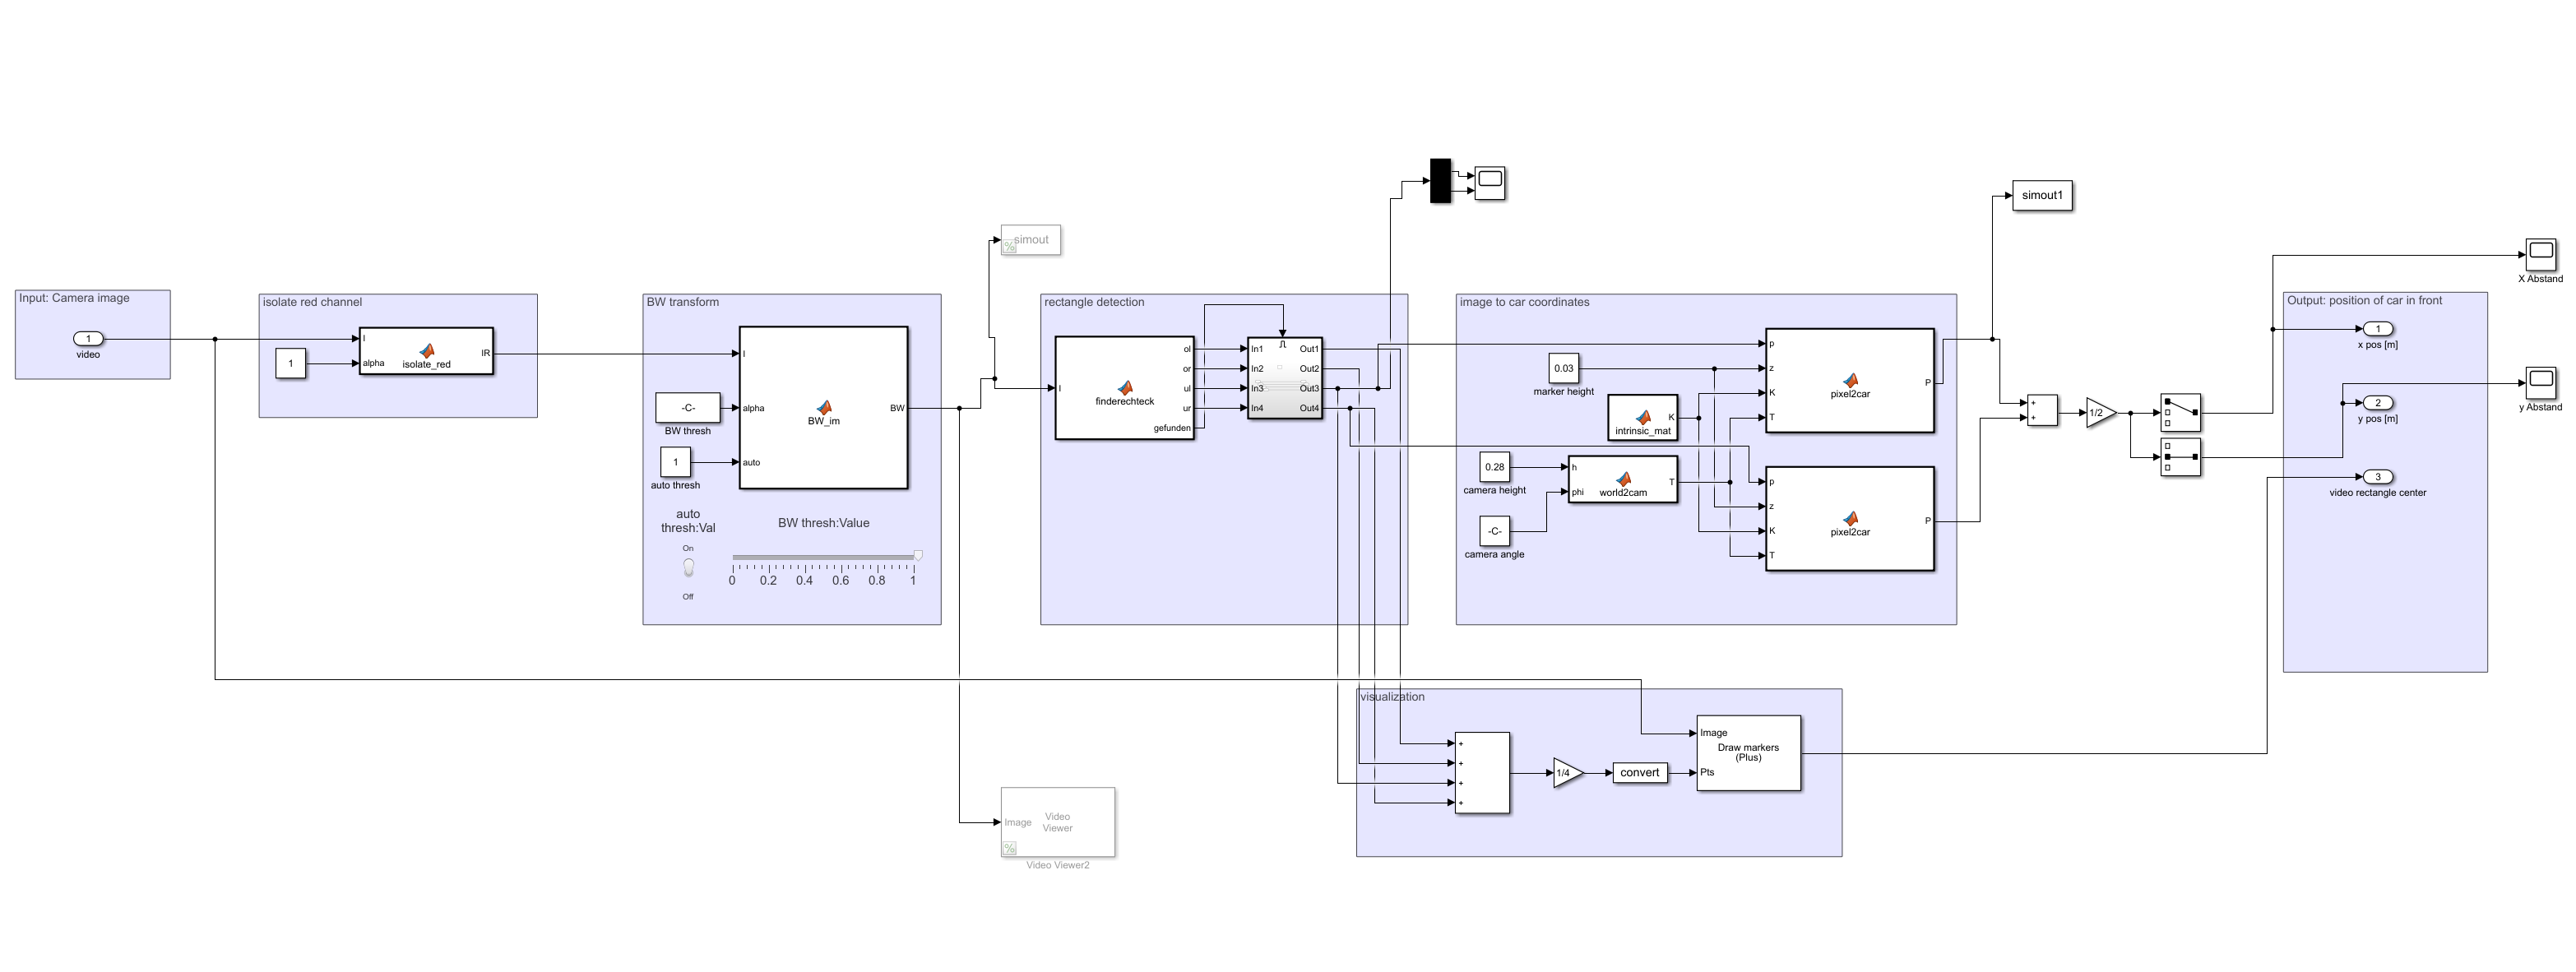
\includegraphics[width=1.1\textwidth]{Simulink.PNG}
	\caption{Abstandsbestimmung Kamera-Objekt in Simulink} 
	\label{img:grafik-dummy}
\end{figure}

\subsection{Abstandsregler}
Der implementierte Abstandsregler nutzt die zuvor berechneten Abstände zum getrackten Objekt. Der Abstand in Fahrtrichtung wird durch \textit{x pos} beschrieben, der Abstand quer zur Fahrtrichtung durch \textit{y pos}. 
Für die Abstandsregelung wird der aktuelle Abstand mit einer Zieldistanz verglichen,  mittels eines P-Regler geregelt und auf Werte zwischen $-0.5$ und $0.5$ begrenzt. 
Um ein Rückwärtsfahren bei Unterschreitung des geforderten Abstands zu gewährleisten, wird bei einem negativen Wert die Drehrichtung des Motors umgedreht. \\

Für die Regelung des Lenkungwinkels wird der gemessene  Querabstand durch eine Verstärkung auf einen Wert zwischen $-1$ und $1$ gebracht. 


\begin{figure}[h]
	\centering
	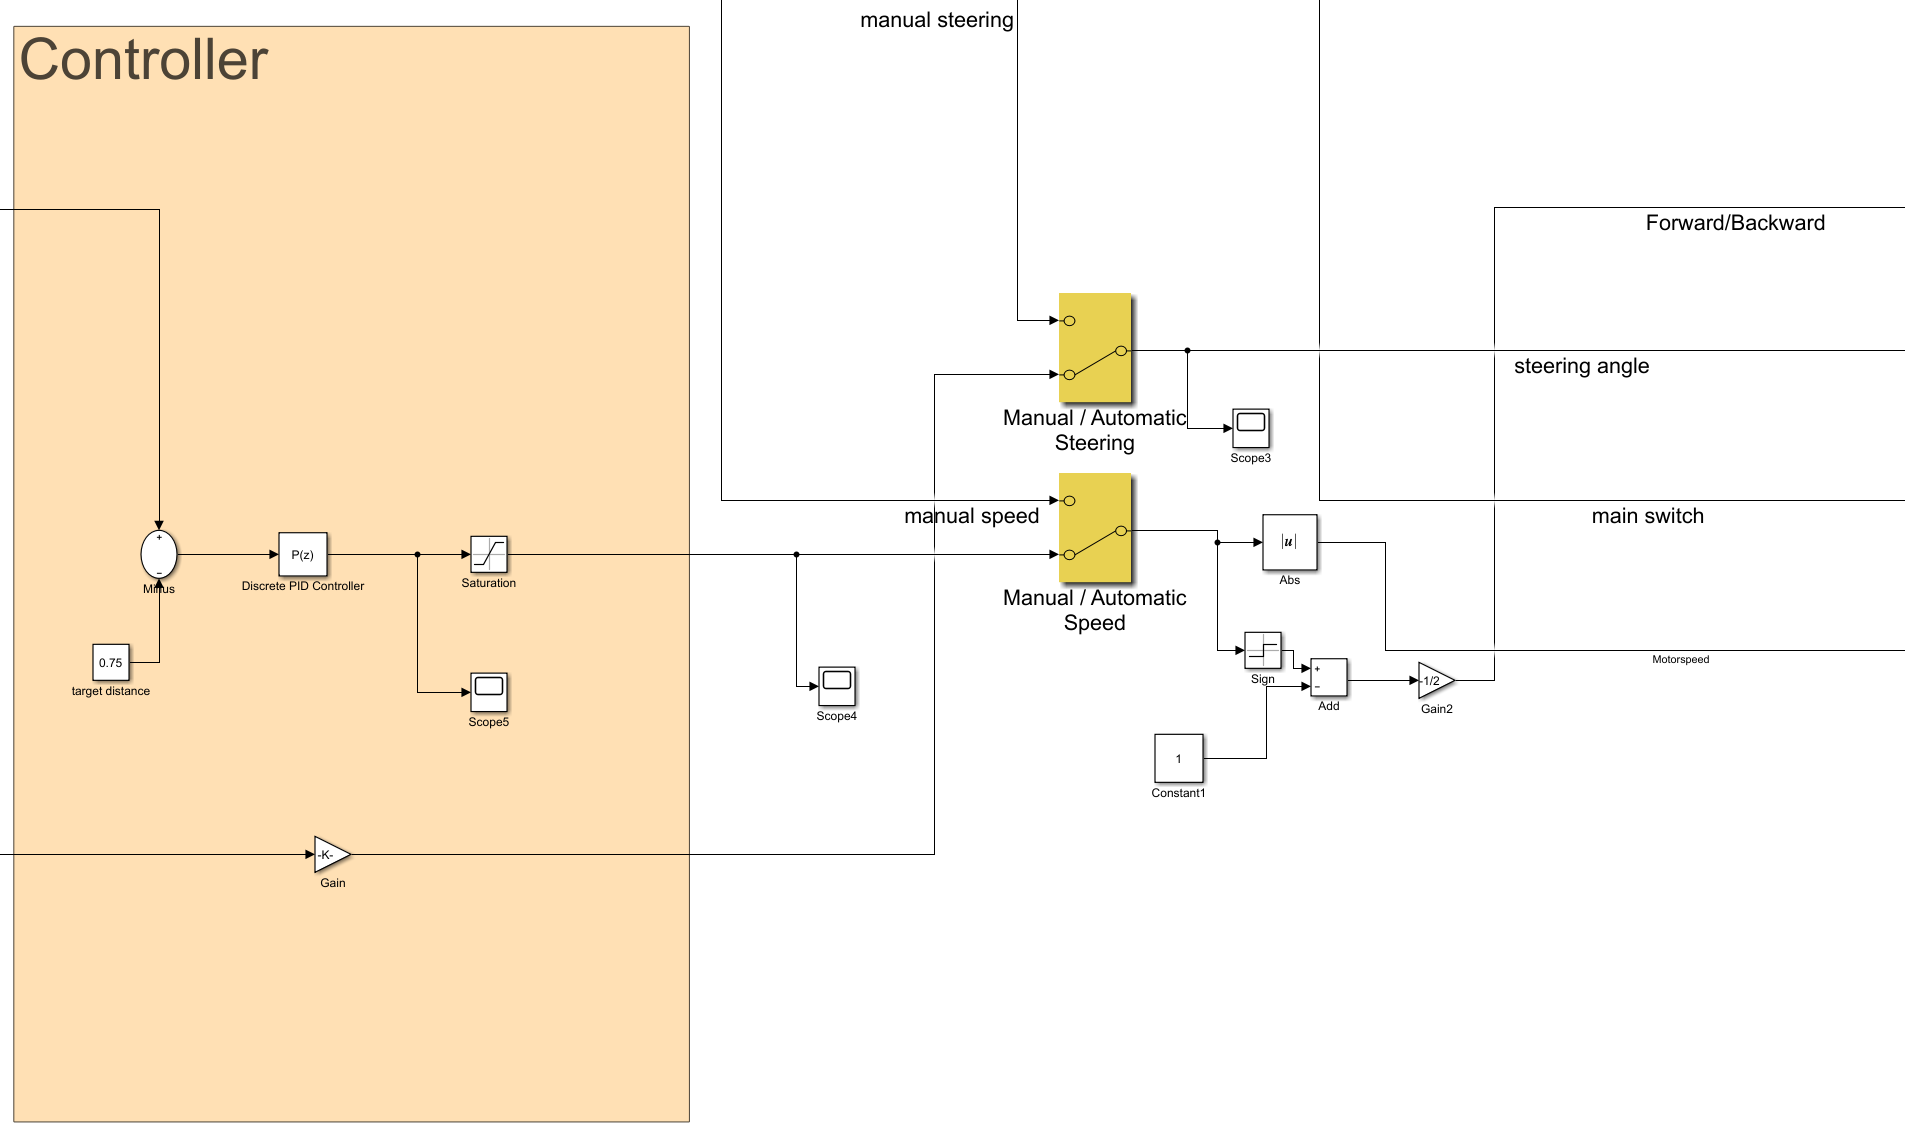
\includegraphics[width=1.1\textwidth]{Controller.PNG}
	\caption{Abstandsregler in Simulink }
	\label{img:grafik-dummy}
\end{figure}
